\documentclass[border=0pt]{standalone}
\usepackage[T1]{fontenc}
\usepackage[tt=false,type1=true]{libertine}
\usepackage{tikz}
\pdfinfoomitdate=1
\pdftrailerid{}
\pdfsuppressptexinfo=15
\definecolor{ink}{HTML}{111111}
\definecolor{muted}{HTML}{555555}
\definecolor{grid}{HTML}{808080}
\definecolor{band}{HTML}{F5F5F5}
\definecolor{white}{HTML}{FFFFFF}
\definecolor{m0}{HTML}{DE8F05}
\definecolor{t0}{HTML}{A66700}
\definecolor{m1}{HTML}{0173B2}
\definecolor{t1}{HTML}{0173B2}
\definecolor{m2}{HTML}{029E73}
\definecolor{t2}{HTML}{00855F}
\definecolor{m3}{HTML}{CC78BC}
\definecolor{t3}{HTML}{A45C96}
\definecolor{m4}{HTML}{D55E00}
\definecolor{t4}{HTML}{C35300}
\begin{document}
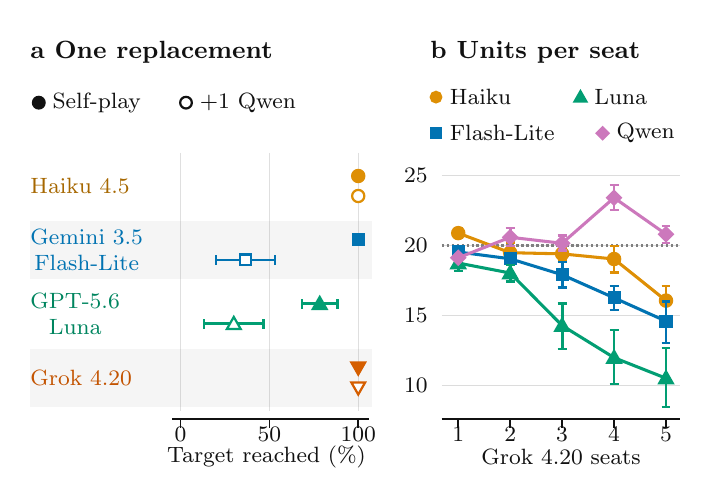
\begin{tikzpicture}[x=1bp,y=-1bp,text=ink,every node/.style={inner sep=0pt,outer sep=0pt,font=\fontsize{8.25}{9.5}\selectfont}]
\path[use as bounding box] (0,0) rectangle (241.1475,159.5);
\node[anchor=west,align=center,text=ink,font=\fontsize{9.2}{10}\selectfont\bfseries] at (1.00000,9.00000) {a  One replacement};
\node[anchor=west,align=center,text=ink,font=\fontsize{9.2}{10}\selectfont\bfseries] at (145.00000,9.00000) {b  Units per seat};
\path[draw=ink,fill=ink,line width=.8bp] (4.00000,27.00000) circle[radius=2.1bp];
\node[anchor=west,align=center,text=ink] at (9.00000,27.00000) {Self-play};
\path[draw=ink,fill=white,line width=.8bp] (57.00000,27.00000) circle[radius=2.1bp];
\node[anchor=west,align=center,text=ink] at (62.00000,27.00000) {+1 Qwen};
\path[draw=m0,fill=m0,line width=0.8bp] (147.00000,25.00000) circle[radius=1.9bp];
\node[anchor=west,align=center,text=ink] at (152.00000,25.00000) {Haiku};
\path[draw=m2,fill=m2,line width=0.8bp] (199.00000,22.87200) -- (201.12800,26.59600) -- (196.87200,26.59600) -- cycle;
\node[anchor=west,align=center,text=ink] at (204.00000,25.00000) {Luna};
\path[draw=m1,fill=m1,line width=0.8bp] (145.30900,36.30900) rectangle (148.69100,39.69100);
\node[anchor=west,align=center,text=ink] at (152.00000,38.00000) {Flash-Lite};
\path[draw=m3,fill=m3,line width=0.8bp] (207.00000,35.87200) -- (209.12800,38.00000) -- (207.00000,40.12800) -- (204.87200,38.00000) -- cycle;
\node[anchor=west,align=center,text=ink] at (212.00000,38.00000) {Qwen};
\node[anchor=west,align=center,text=t0] at (1.00000,57.00000) {Haiku 4.5};
\fill[band] (1.00000,69.50000) rectangle (124.00000,90.50000);
\node[anchor=west,align=center,text=t1] at (1.00000,80.00000) {Gemini 3.5\\Flash-Lite};
\node[anchor=west,align=center,text=t2] at (1.00000,103.00000) {GPT-5.6\\Luna};
\fill[band] (1.00000,115.50000) rectangle (124.00000,136.50000);
\node[anchor=west,align=center,text=t4] at (1.00000,126.00000) {Grok 4.20};
\draw[draw=grid,line width=0.5bp,opacity=0.25] (55.00000,45.00000) -- (55.00000,138.00000);
\draw[draw=grid,line width=0.5bp,opacity=0.25] (87.00000,45.00000) -- (87.00000,138.00000);
\draw[draw=grid,line width=0.5bp,opacity=0.25] (119.00000,45.00000) -- (119.00000,138.00000);
\draw[draw=m0,line width=1.0bp,opacity=1] (119.00000,53.40000) -- (119.00000,53.40000);
\draw[draw=m0,line width=0.8bp,opacity=1] (119.00000,51.70000) -- (119.00000,55.10000);
\draw[draw=m0,line width=0.8bp,opacity=1] (119.00000,51.70000) -- (119.00000,55.10000);
\path[draw=m0,fill=m0,line width=0.8bp] (119.00000,53.40000) circle[radius=2.2bp];
\draw[draw=m0,line width=1.0bp,opacity=1] (119.00000,60.60000) -- (119.00000,60.60000);
\draw[draw=m0,line width=0.8bp,opacity=1] (119.00000,58.90000) -- (119.00000,62.30000);
\draw[draw=m0,line width=0.8bp,opacity=1] (119.00000,58.90000) -- (119.00000,62.30000);
\path[draw=m0,fill=white,line width=0.8bp] (119.00000,60.60000) circle[radius=2.2bp];
\draw[draw=m1,line width=1.0bp,opacity=1] (119.00000,76.40000) -- (119.00000,76.40000);
\draw[draw=m1,line width=0.8bp,opacity=1] (119.00000,74.70000) -- (119.00000,78.10000);
\draw[draw=m1,line width=0.8bp,opacity=1] (119.00000,74.70000) -- (119.00000,78.10000);
\path[draw=m1,fill=m1,line width=0.8bp] (117.04200,74.44200) rectangle (120.95800,78.35800);
\draw[draw=m1,line width=1.0bp,opacity=1] (67.80000,83.60000) -- (89.13333,83.60000);
\draw[draw=m1,line width=0.8bp,opacity=1] (67.80000,81.90000) -- (67.80000,85.30000);
\draw[draw=m1,line width=0.8bp,opacity=1] (89.13333,81.90000) -- (89.13333,85.30000);
\path[draw=m1,fill=white,line width=0.8bp] (76.50867,81.64200) rectangle (80.42467,85.55800);
\draw[draw=m2,line width=1.0bp,opacity=1] (98.73333,99.40000) -- (111.53333,99.40000);
\draw[draw=m2,line width=0.8bp,opacity=1] (98.73333,97.70000) -- (98.73333,101.10000);
\draw[draw=m2,line width=0.8bp,opacity=1] (111.53333,97.70000) -- (111.53333,101.10000);
\path[draw=m2,fill=m2,line width=0.8bp] (105.13333,96.93600) -- (107.59733,101.24800) -- (102.66933,101.24800) -- cycle;
\draw[draw=m2,line width=1.0bp,opacity=1] (63.53333,106.60000) -- (84.86667,106.60000);
\draw[draw=m2,line width=0.8bp,opacity=1] (63.53333,104.90000) -- (63.53333,108.30000);
\draw[draw=m2,line width=0.8bp,opacity=1] (84.86667,104.90000) -- (84.86667,108.30000);
\path[draw=m2,fill=white,line width=0.8bp] (74.20000,104.13600) -- (76.66400,108.44800) -- (71.73600,108.44800) -- cycle;
\draw[draw=m4,line width=1.0bp,opacity=1] (119.00000,122.40000) -- (119.00000,122.40000);
\draw[draw=m4,line width=0.8bp,opacity=1] (119.00000,120.70000) -- (119.00000,124.10000);
\draw[draw=m4,line width=0.8bp,opacity=1] (119.00000,120.70000) -- (119.00000,124.10000);
\path[draw=m4,fill=m4,line width=0.8bp] (119.00000,124.86400) -- (121.46400,120.55200) -- (116.53600,120.55200) -- cycle;
\draw[draw=m4,line width=1.0bp,opacity=1] (119.00000,129.60000) -- (119.00000,129.60000);
\draw[draw=m4,line width=0.8bp,opacity=1] (119.00000,127.90000) -- (119.00000,131.30000);
\draw[draw=m4,line width=0.8bp,opacity=1] (119.00000,127.90000) -- (119.00000,131.30000);
\path[draw=m4,fill=white,line width=0.8bp] (119.00000,132.06400) -- (121.46400,127.75200) -- (116.53600,127.75200) -- cycle;
\draw[draw=grid,line width=0.5bp,opacity=0.28] (149.00000,128.90000) -- (235.00000,128.90000);
\node[anchor=east,align=center,text=ink] at (144.00000,128.90000) {10};
\draw[draw=grid,line width=0.5bp,opacity=0.28] (149.00000,103.65000) -- (235.00000,103.65000);
\node[anchor=east,align=center,text=ink] at (144.00000,103.65000) {15};
\draw[draw=grid,line width=0.5bp,opacity=0.28] (149.00000,78.40000) -- (235.00000,78.40000);
\node[anchor=east,align=center,text=ink] at (144.00000,78.40000) {20};
\draw[draw=grid,line width=0.5bp,opacity=0.28] (149.00000,53.15000) -- (235.00000,53.15000);
\node[anchor=east,align=center,text=ink] at (144.00000,53.15000) {25};
\draw[draw=grid,line width=0.8bp,opacity=1,densely dotted] (149.00000,78.40000) -- (235.00000,78.40000);
\draw[draw=m0,line width=1.1bp,opacity=1] (155.00000,73.95600) -- (173.70000,81.00917);
\draw[draw=m0,line width=1.1bp,opacity=1] (173.70000,81.00917) -- (192.40000,81.43000);
\draw[draw=m0,line width=1.1bp,opacity=1] (192.40000,81.43000) -- (211.10000,83.28167);
\draw[draw=m0,line width=1.1bp,opacity=1] (211.10000,83.28167) -- (229.80000,98.26333);
\draw[draw=m0,line width=1.0bp,opacity=1] (155.00000,72.20533) -- (155.00000,75.70667);
\draw[draw=m0,line width=0.8bp,opacity=1] (153.40000,72.20533) -- (156.60000,72.20533);
\draw[draw=m0,line width=0.8bp,opacity=1] (153.40000,75.70667) -- (156.60000,75.70667);
\path[draw=m0,fill=m0,line width=0.8bp] (155.00000,73.95600) circle[radius=2.2bp];
\draw[draw=m0,line width=1.0bp,opacity=1] (173.70000,77.30583) -- (173.70000,84.46000);
\draw[draw=m0,line width=0.8bp,opacity=1] (172.10000,77.30583) -- (175.30000,77.30583);
\draw[draw=m0,line width=0.8bp,opacity=1] (172.10000,84.46000) -- (175.30000,84.46000);
\path[draw=m0,fill=m0,line width=0.8bp] (173.70000,81.00917) circle[radius=2.2bp];
\draw[draw=m0,line width=1.0bp,opacity=1] (192.40000,79.29778) -- (192.40000,83.56222);
\draw[draw=m0,line width=0.8bp,opacity=1] (190.80000,79.29778) -- (194.00000,79.29778);
\draw[draw=m0,line width=0.8bp,opacity=1] (190.80000,83.56222) -- (194.00000,83.56222);
\path[draw=m0,fill=m0,line width=0.8bp] (192.40000,81.43000) circle[radius=2.2bp];
\draw[draw=m0,line width=1.0bp,opacity=1] (211.10000,78.56833) -- (211.10000,88.16333);
\draw[draw=m0,line width=0.8bp,opacity=1] (209.50000,78.56833) -- (212.70000,78.56833);
\draw[draw=m0,line width=0.8bp,opacity=1] (209.50000,88.16333) -- (212.70000,88.16333);
\path[draw=m0,fill=m0,line width=0.8bp] (211.10000,83.28167) circle[radius=2.2bp];
\draw[draw=m0,line width=1.0bp,opacity=1] (229.80000,92.87667) -- (229.80000,104.32333);
\draw[draw=m0,line width=0.8bp,opacity=1] (228.20000,92.87667) -- (231.40000,92.87667);
\draw[draw=m0,line width=0.8bp,opacity=1] (228.20000,104.32333) -- (231.40000,104.32333);
\path[draw=m0,fill=m0,line width=0.8bp] (229.80000,98.26333) circle[radius=2.2bp];
\draw[draw=m1,line width=1.1bp,opacity=1] (155.00000,80.75667) -- (173.70000,83.19750);
\draw[draw=m1,line width=1.1bp,opacity=1] (173.70000,83.19750) -- (192.40000,88.94889);
\draw[draw=m1,line width=1.1bp,opacity=1] (192.40000,88.94889) -- (211.10000,97.25333);
\draw[draw=m1,line width=1.1bp,opacity=1] (211.10000,97.25333) -- (229.80000,105.67000);
\draw[draw=m1,line width=1.0bp,opacity=1] (155.00000,79.14067) -- (155.00000,82.50733);
\draw[draw=m1,line width=0.8bp,opacity=1] (153.40000,79.14067) -- (156.60000,79.14067);
\draw[draw=m1,line width=0.8bp,opacity=1] (153.40000,82.50733) -- (156.60000,82.50733);
\path[draw=m1,fill=m1,line width=0.8bp] (153.04200,78.79867) rectangle (156.95800,82.71467);
\draw[draw=m1,line width=1.0bp,opacity=1] (173.70000,81.59833) -- (173.70000,84.88083);
\draw[draw=m1,line width=0.8bp,opacity=1] (172.10000,81.59833) -- (175.30000,81.59833);
\draw[draw=m1,line width=0.8bp,opacity=1] (172.10000,84.88083) -- (175.30000,84.88083);
\path[draw=m1,fill=m1,line width=0.8bp] (171.74200,81.23950) rectangle (175.65800,85.15550);
\draw[draw=m1,line width=1.0bp,opacity=1] (192.40000,84.46000) -- (192.40000,93.55281);
\draw[draw=m1,line width=0.8bp,opacity=1] (190.80000,84.46000) -- (194.00000,84.46000);
\draw[draw=m1,line width=0.8bp,opacity=1] (190.80000,93.55281) -- (194.00000,93.55281);
\path[draw=m1,fill=m1,line width=0.8bp] (190.44200,86.99089) rectangle (194.35800,90.90689);
\draw[draw=m1,line width=1.0bp,opacity=1] (211.10000,92.87667) -- (211.10000,101.63000);
\draw[draw=m1,line width=0.8bp,opacity=1] (209.50000,92.87667) -- (212.70000,92.87667);
\draw[draw=m1,line width=0.8bp,opacity=1] (209.50000,101.63000) -- (212.70000,101.63000);
\path[draw=m1,fill=m1,line width=0.8bp] (209.14200,95.29533) rectangle (213.05800,99.21133);
\draw[draw=m1,line width=1.0bp,opacity=1] (229.80000,98.60000) -- (229.80000,113.41333);
\draw[draw=m1,line width=0.8bp,opacity=1] (228.20000,98.60000) -- (231.40000,98.60000);
\draw[draw=m1,line width=0.8bp,opacity=1] (228.20000,113.41333) -- (231.40000,113.41333);
\path[draw=m1,fill=m1,line width=0.8bp] (227.84200,103.71200) rectangle (231.75800,107.62800);
\draw[draw=m2,line width=1.1bp,opacity=1] (155.00000,84.72933) -- (173.70000,88.33167);
\draw[draw=m2,line width=1.1bp,opacity=1] (173.70000,88.33167) -- (192.40000,107.24111);
\draw[draw=m2,line width=1.1bp,opacity=1] (192.40000,107.24111) -- (211.10000,118.80000);
\draw[draw=m2,line width=1.1bp,opacity=1] (211.10000,118.80000) -- (229.80000,126.20667);
\draw[draw=m2,line width=1.0bp,opacity=1] (155.00000,82.03600) -- (155.00000,87.69200);
\draw[draw=m2,line width=0.8bp,opacity=1] (153.40000,82.03600) -- (156.60000,82.03600);
\draw[draw=m2,line width=0.8bp,opacity=1] (153.40000,87.69200) -- (156.60000,87.69200);
\path[draw=m2,fill=m2,line width=0.8bp] (155.00000,82.26533) -- (157.46400,86.57733) -- (152.53600,86.57733) -- cycle;
\draw[draw=m2,line width=1.0bp,opacity=1] (173.70000,85.30167) -- (173.70000,91.36167);
\draw[draw=m2,line width=0.8bp,opacity=1] (172.10000,85.30167) -- (175.30000,85.30167);
\draw[draw=m2,line width=0.8bp,opacity=1] (172.10000,91.36167) -- (175.30000,91.36167);
\path[draw=m2,fill=m2,line width=0.8bp] (173.70000,85.86767) -- (176.16400,90.17967) -- (171.23600,90.17967) -- cycle;
\draw[draw=m2,line width=1.0bp,opacity=1] (192.40000,99.27333) -- (192.40000,115.65778);
\draw[draw=m2,line width=0.8bp,opacity=1] (190.80000,99.27333) -- (194.00000,99.27333);
\draw[draw=m2,line width=0.8bp,opacity=1] (190.80000,115.65778) -- (194.00000,115.65778);
\path[draw=m2,fill=m2,line width=0.8bp] (192.40000,104.77711) -- (194.86400,109.08911) -- (189.93600,109.08911) -- cycle;
\draw[draw=m2,line width=1.0bp,opacity=1] (211.10000,108.86833) -- (211.10000,128.22667);
\draw[draw=m2,line width=0.8bp,opacity=1] (209.50000,108.86833) -- (212.70000,108.86833);
\draw[draw=m2,line width=0.8bp,opacity=1] (209.50000,128.22667) -- (212.70000,128.22667);
\path[draw=m2,fill=m2,line width=0.8bp] (211.10000,116.33600) -- (213.56400,120.64800) -- (208.63600,120.64800) -- cycle;
\draw[draw=m2,line width=1.0bp,opacity=1] (229.80000,115.43333) -- (229.80000,136.64333);
\draw[draw=m2,line width=0.8bp,opacity=1] (228.20000,115.43333) -- (231.40000,115.43333);
\draw[draw=m2,line width=0.8bp,opacity=1] (228.20000,136.64333) -- (231.40000,136.64333);
\path[draw=m2,fill=m2,line width=0.8bp] (229.80000,123.74267) -- (232.26400,128.05467) -- (227.33600,128.05467) -- cycle;
\draw[draw=m3,line width=1.1bp,opacity=1] (155.00000,82.84400) -- (173.70000,75.45417);
\draw[draw=m3,line width=1.1bp,opacity=1] (173.70000,75.45417) -- (192.40000,77.61444);
\draw[draw=m3,line width=1.1bp,opacity=1] (192.40000,77.61444) -- (211.10000,61.23000);
\draw[draw=m3,line width=1.1bp,opacity=1] (211.10000,61.23000) -- (229.80000,74.36000);
\draw[draw=m3,line width=1.0bp,opacity=1] (155.00000,81.96867) -- (155.00000,83.71933);
\draw[draw=m3,line width=0.8bp,opacity=1] (153.40000,81.96867) -- (156.60000,81.96867);
\draw[draw=m3,line width=0.8bp,opacity=1] (153.40000,83.71933) -- (156.60000,83.71933);
\path[draw=m3,fill=m3,line width=0.8bp] (155.00000,80.38000) -- (157.46400,82.84400) -- (155.00000,85.30800) -- (152.53600,82.84400) -- cycle;
\draw[draw=m3,line width=1.0bp,opacity=1] (173.70000,72.00333) -- (173.70000,78.73667);
\draw[draw=m3,line width=0.8bp,opacity=1] (172.10000,72.00333) -- (175.30000,72.00333);
\draw[draw=m3,line width=0.8bp,opacity=1] (172.10000,78.73667) -- (175.30000,78.73667);
\path[draw=m3,fill=m3,line width=0.8bp] (173.70000,72.99017) -- (176.16400,75.45417) -- (173.70000,77.91817) -- (171.23600,75.45417) -- cycle;
\draw[draw=m3,line width=1.0bp,opacity=1] (192.40000,74.80889) -- (192.40000,80.19556);
\draw[draw=m3,line width=0.8bp,opacity=1] (190.80000,74.80889) -- (194.00000,74.80889);
\draw[draw=m3,line width=0.8bp,opacity=1] (190.80000,80.19556) -- (194.00000,80.19556);
\path[draw=m3,fill=m3,line width=0.8bp] (192.40000,75.15044) -- (194.86400,77.61444) -- (192.40000,80.07844) -- (189.93600,77.61444) -- cycle;
\draw[draw=m3,line width=1.0bp,opacity=1] (211.10000,56.68500) -- (211.10000,65.60667);
\draw[draw=m3,line width=0.8bp,opacity=1] (209.50000,56.68500) -- (212.70000,56.68500);
\draw[draw=m3,line width=0.8bp,opacity=1] (209.50000,65.60667) -- (212.70000,65.60667);
\path[draw=m3,fill=m3,line width=0.8bp] (211.10000,58.76600) -- (213.56400,61.23000) -- (211.10000,63.69400) -- (208.63600,61.23000) -- cycle;
\draw[draw=m3,line width=1.0bp,opacity=1] (229.80000,71.33000) -- (229.80000,77.39000);
\draw[draw=m3,line width=0.8bp,opacity=1] (228.20000,71.33000) -- (231.40000,71.33000);
\draw[draw=m3,line width=0.8bp,opacity=1] (228.20000,77.39000) -- (231.40000,77.39000);
\path[draw=m3,fill=m3,line width=0.8bp] (229.80000,71.89600) -- (232.26400,74.36000) -- (229.80000,76.82400) -- (227.33600,74.36000) -- cycle;
\draw[draw=ink,line width=0.7bp,opacity=1] (52.00000,141.00000) -- (123.00000,141.00000);
\draw[draw=ink,line width=0.7bp,opacity=1] (149.00000,141.00000) -- (235.00000,141.00000);
\draw[draw=ink,line width=0.6bp,opacity=1] (55.00000,141.00000) -- (55.00000,144.00000);
\node[anchor=center,align=center,text=ink] at (55.00000,146.50000) {0};
\draw[draw=ink,line width=0.6bp,opacity=1] (87.00000,141.00000) -- (87.00000,144.00000);
\node[anchor=center,align=center,text=ink] at (87.00000,146.50000) {50};
\draw[draw=ink,line width=0.6bp,opacity=1] (119.00000,141.00000) -- (119.00000,144.00000);
\node[anchor=center,align=center,text=ink] at (119.00000,146.50000) {100};
\draw[draw=ink,line width=0.6bp,opacity=1] (155.00000,141.00000) -- (155.00000,144.00000);
\node[anchor=center,align=center,text=ink] at (155.00000,146.50000) {1};
\draw[draw=ink,line width=0.6bp,opacity=1] (173.70000,141.00000) -- (173.70000,144.00000);
\node[anchor=center,align=center,text=ink] at (173.70000,146.50000) {2};
\draw[draw=ink,line width=0.6bp,opacity=1] (192.40000,141.00000) -- (192.40000,144.00000);
\node[anchor=center,align=center,text=ink] at (192.40000,146.50000) {3};
\draw[draw=ink,line width=0.6bp,opacity=1] (211.10000,141.00000) -- (211.10000,144.00000);
\node[anchor=center,align=center,text=ink] at (211.10000,146.50000) {4};
\draw[draw=ink,line width=0.6bp,opacity=1] (229.80000,141.00000) -- (229.80000,144.00000);
\node[anchor=center,align=center,text=ink] at (229.80000,146.50000) {5};
\node[anchor=center,align=center,text=ink] at (86.00000,154.50000) {Target reached (\%)};
\node[anchor=center,align=center,text=ink] at (192.00000,154.50000) {Grok 4.20 seats};
\end{tikzpicture}
\end{document}
